\documentclass[english]{tktltiki}
\usepackage[pdftex]{graphicx}
\usepackage{subfigure}
\usepackage{url}
\usepackage{enumerate}
\begin{document}
%\doublespacing
%\singlespacing
\onehalfspacing

\title{Advanced course in Machine Learning - Week 1}
\author{P�ter Ivanics}
\date{\today}

\maketitle

\section{Background information}

\begin{enumerate}[a)]
	\item I have taken only the "Introduction to Machine Learning" course during the Autumn 2016 semester at University of Helsinki. I have not taken any courses in this field at the University of Helsinki otherwise. Nevertheless, during my first Bachelor degree I have taken a course in Probability and Statistics at �buda University in 2011. 
	\item I have some knowledge in statistics and I am familiar with the basic concepts, but advanced topics are fairly unknown to me as it turned out during the course last semester - I would say around 3
	\item For similar reasons, around 3
	\item The reason why I have taken this course is that I greatly enjoyed the preliminary course mentioned above. Additionally, I have started studying on this master programme to enhance my knowledge in this topic and I believe this is a direction to which I should specialize and dig deeper into. 
	\item I would like to learn about the application fields of machine learning and understand the capabilities. I would like to know what kind of open APIs exist in case I would have to use some classifier for my work or projects. Additionally, I am more than happy to implement some "common" algorithms myself and see how they perform on different datasets and distributions. The best outcome from this course for me personally would be the knowledge, what I can apply straight to my work as a software developer and come up with a suggestion how Machine Learning could be utilized at the company I am working for.
\end{enumerate}

\section{Expectations}
\begin{center}
	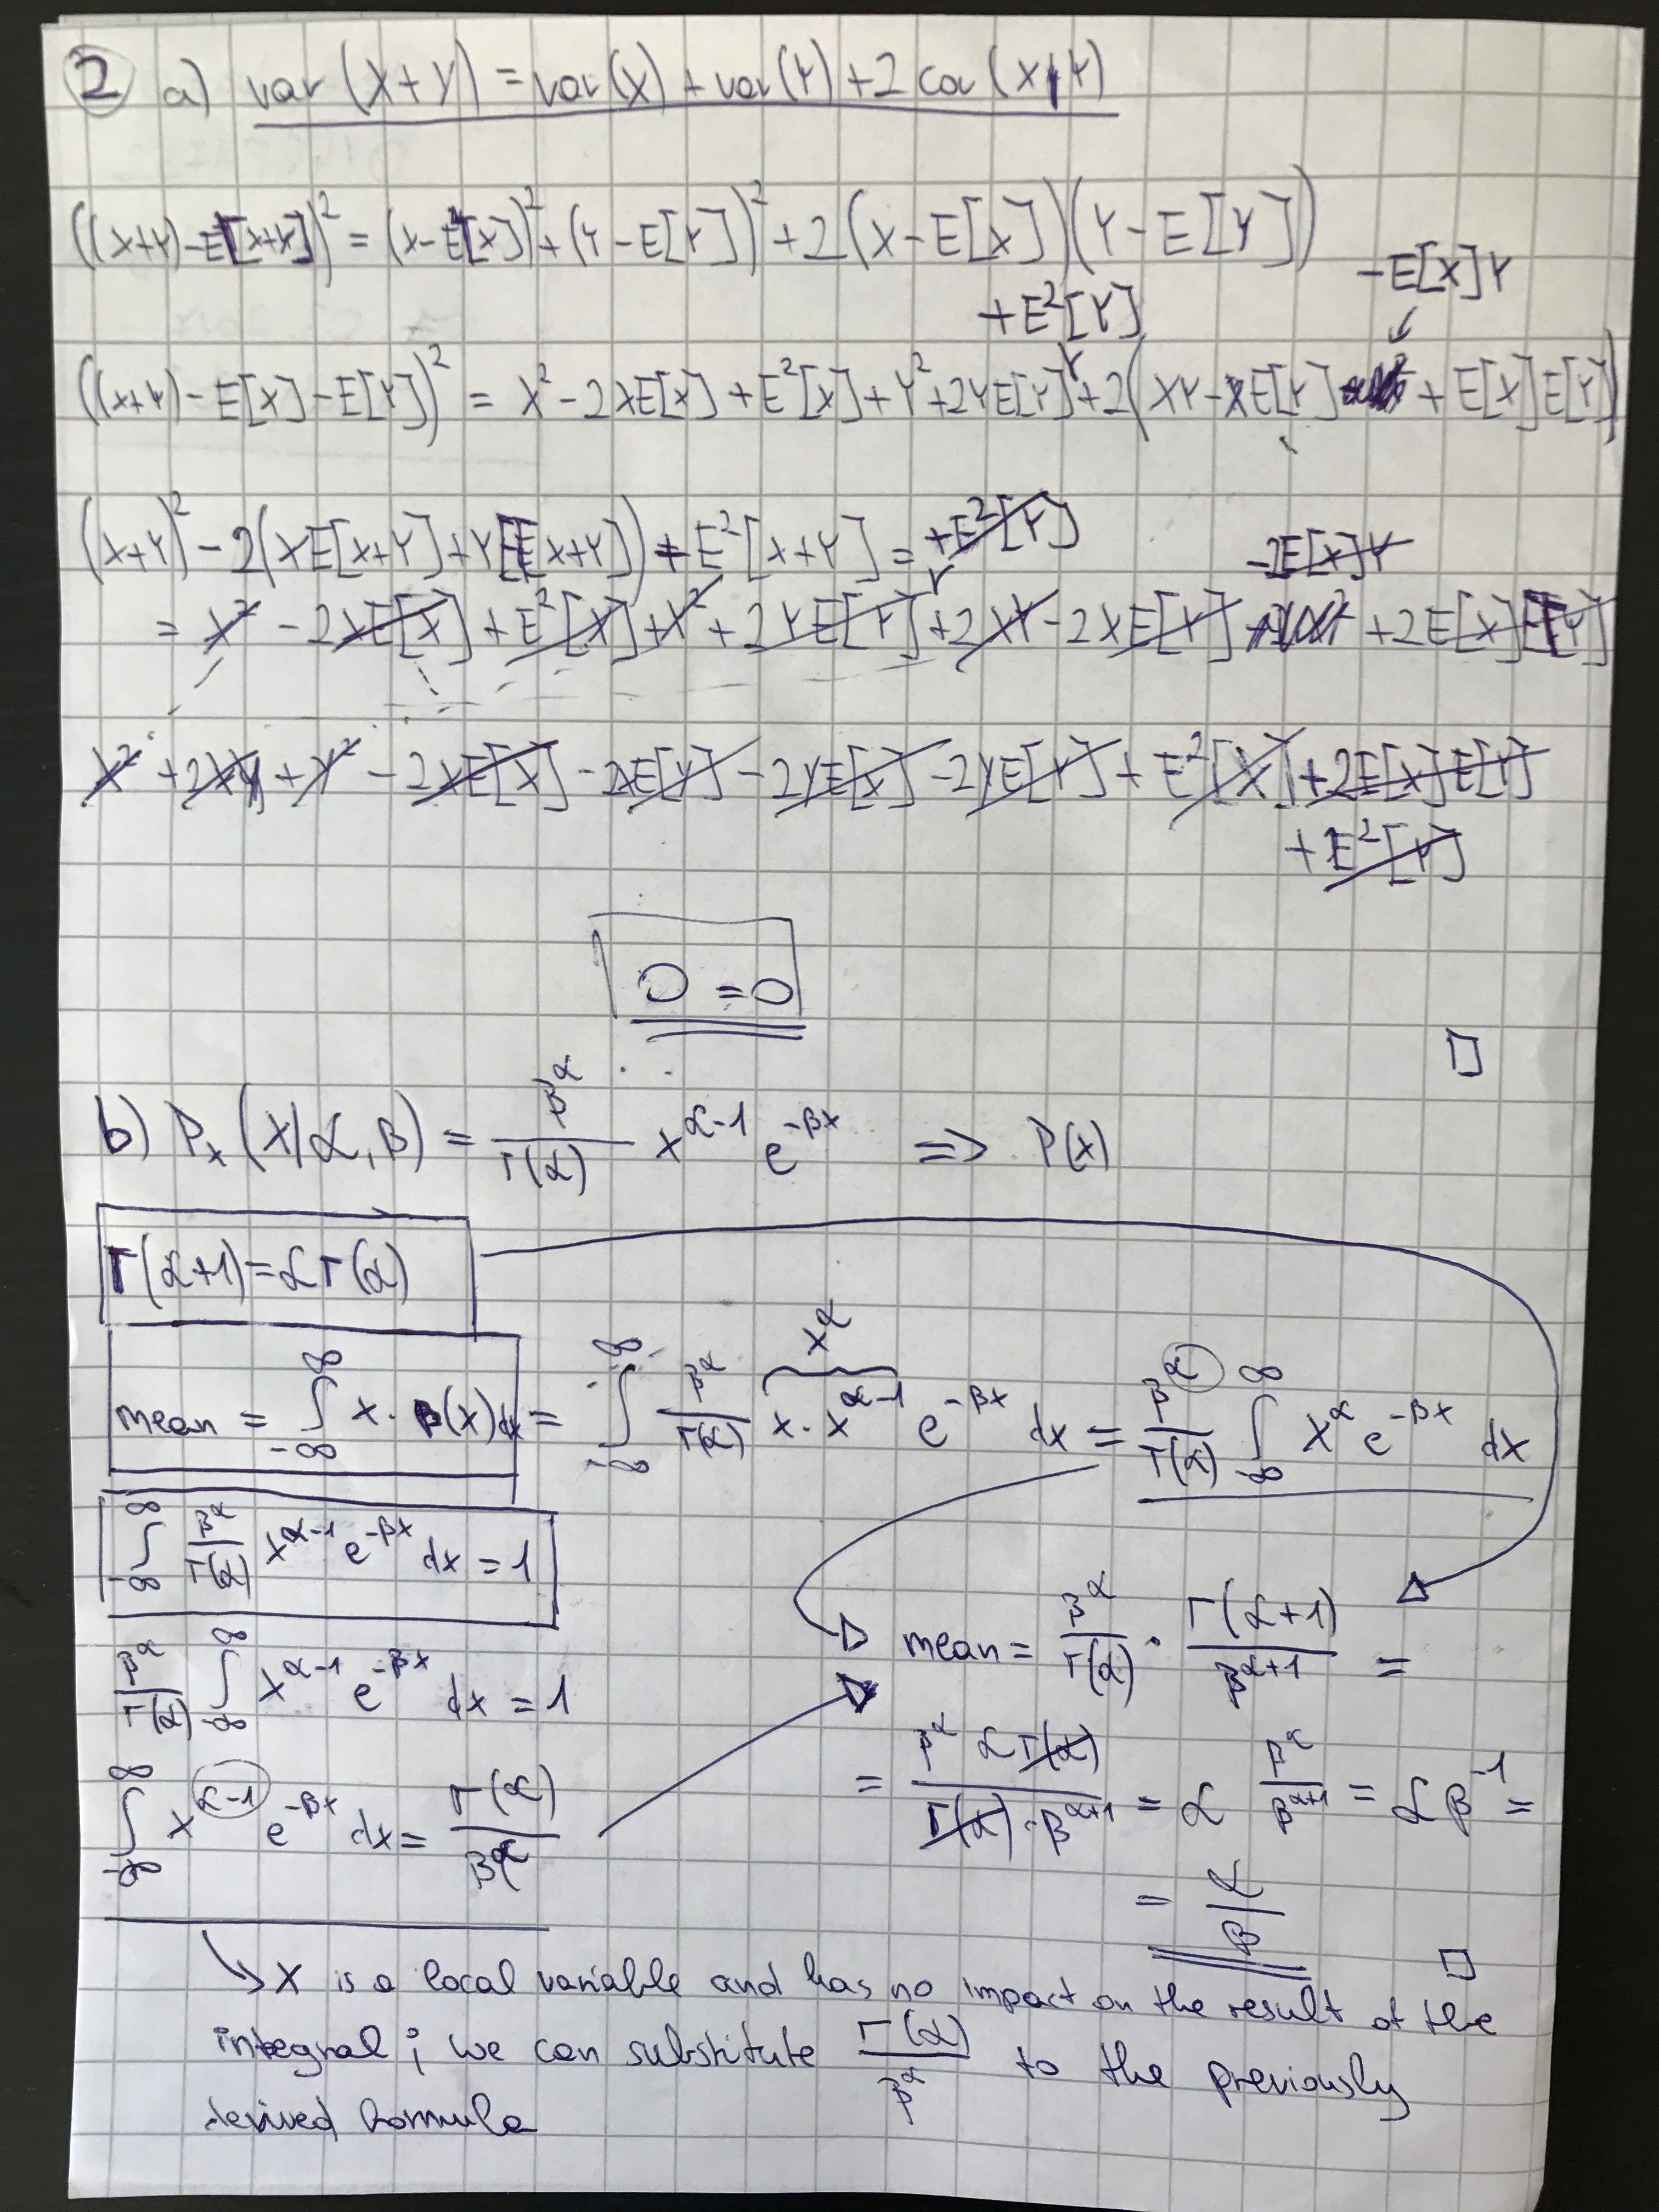
\includegraphics[width=1\textwidth]{images/IMG_0074.jpg}
\end{center}

\section{Eigen-value decomposition}
\begin{enumerate}
	\item After loading the dataset we can see that the number of observations (rows) in the dataset is D=200 and the number of dimensions (columns) is N=5. 
	\item The Eigenvalues of the covariance matrix \textbf{X} are, as follows: 
	\begin{center}
		$[2.012649572, 0.222861976, 0.142902106, 0.010428670, 0.009259117]$
	\end{center}
	\item After reducing the data to the $L=2$ first eigenvectors, it is reduced to two dimensions. A plot of this dataset is displayed on the figure below. 
	
	\begin{center}
		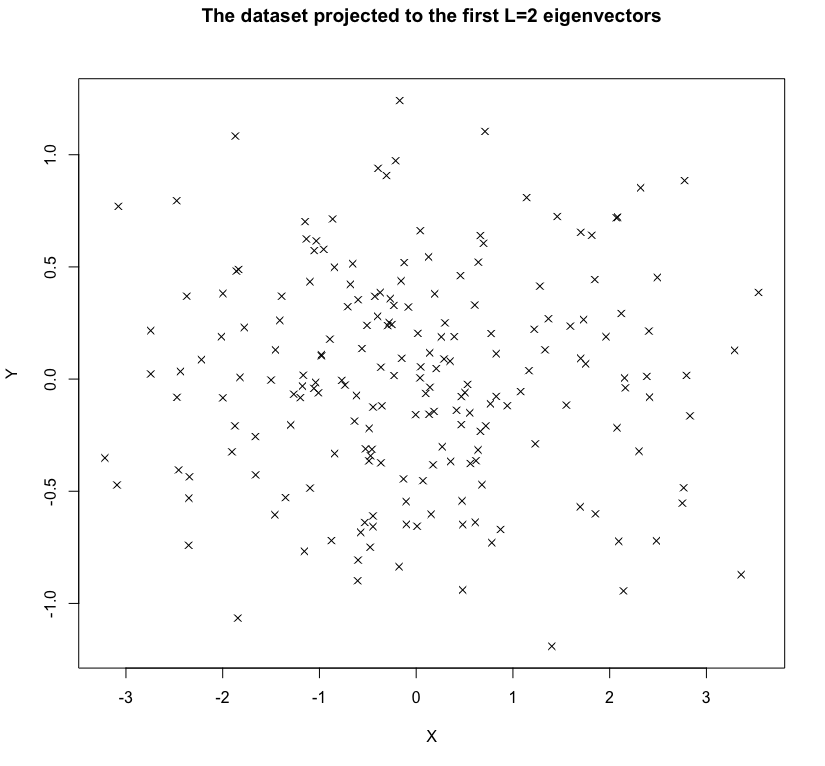
\includegraphics[width=0.75\textwidth]{images/first_two_eigenvectors.png}
	\end{center}
	\item The reconstruction error for L=2,3,4,5 is displayed on the figure below. 
	\begin{center}
		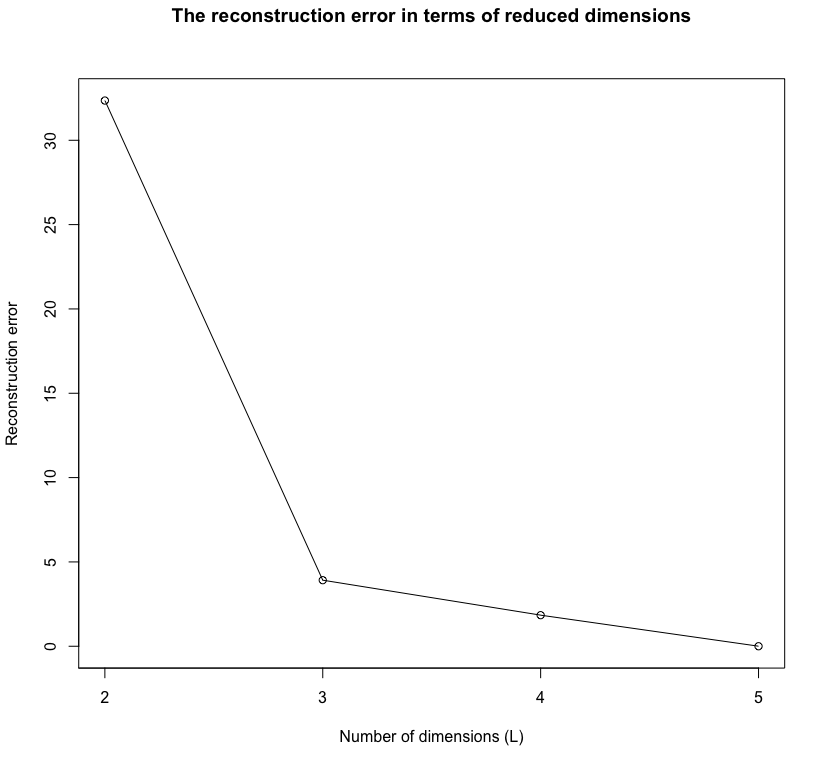
\includegraphics[width=0.75\textwidth]{images/reconstruction_error.png}
	\end{center}
\end{enumerate}
\section{Derivatives, gradients and all that}

\lastpage

\end{document}


